\section{Remote Procedural Call (RPC)}
\label{RPCBackgroundSection} 
RPC is used to uniformly call a procedure that is on a different machine, or on the same machine but on different processes. RPC is implemented on top of a transmission protocol and should work regardless of the communication method being used. For example, we could use TCP/IP for network communications, or any Inter-Process Communication (IPC) method if the caller and callee are on the same machine but in different processes. Normally, RPC implementations would consist of the following steps, as shown in Figure \ref{fig:rpc-components}.

\begin{enumerate}
  \item The caller code is written normally, and so is the server code, but the stubs are automatically generated using interface definition files.
  \item When the remote call is made, it calls the user stub which packs the parameters and function call information into a packet.
  \item The packet gets transferred to its destination (either across the network as in Figure \ref{fig:rpc-components}, or across the processes on the same machine using IPC). This is done through the RPCRuntime, which is a library that works on both ends (caller and callee) to handle communication details.
  \item The packet is received at the callee end by the RPCRuntime. It is then passed on to the server stub.
  \item The arguments and function call information are unpacked and a normal call is made to the actual procedure.
  \item When the procedure returns, it is passed back to the server stub where it is packed and transmitted back to the caller, which unpacks it and uses the result.
\end{enumerate}

\begin{figure}
    \centering
    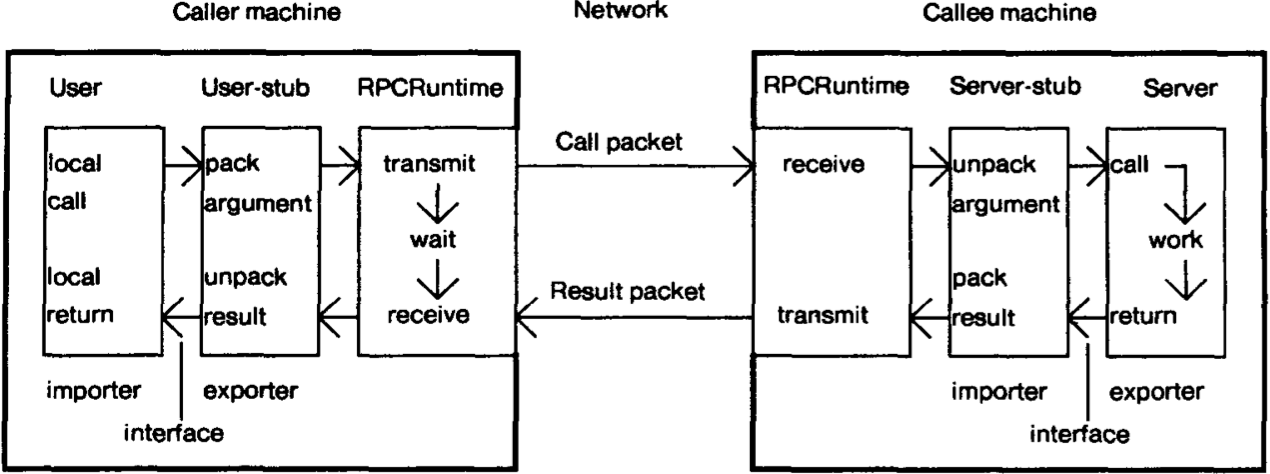
\includegraphics[bb=0 0 1270 474, width=\textwidth]{RPCDiagram_ImplementingRPC_ADBirrell_BJNelson.png} 
    \caption{The basic components of an RPC framework, from \cite{birrell1984implementing}}
    \label{fig:rpc-components}
\end{figure}

\subsection{The role of the RPCRuntime}
\label{RPCRuntimeBackgroundSection} 
The RPCRuntime is responsible for carrying out the actual communication of the RPC call information between the caller and the callee. It exists both in the caller and callee endpoints. When the caller makes a RPC call, the information is sent from the RPCRuntime sitting in the caller side, and is received by the RPCRuntime in the callee side. When the callee returns, the return data is sent from the callee's RPCRuntime to the caller's RPCRuntime.

In order to keep the context of a remote call, the RPCRuntime also sends some extra meta data along with the arguments. This meta data includes:

\begin{enumerate}
	\item A call identifier. This is used for two reasons:
	\begin{enumerate}
		\item To check if the call has already been made (i.e. to ensure no duplicate calls)
		\item To match the return value of the callee with the correct caller.
	\end{enumerate}
	\item The name of the procedure the caller is calling.
	\item The arguments (parameters) we wish to pass to the remote procedure.
\end{enumerate}

The RPCRuntime on the caller side maintains a store of call identifiers that are currently in progress. When the remote functions return, they send the same call identifier along with the return value. That call identifier is then removed from the caller's store to indicate that the remote call has completed. The call identifier is also used to implement the call semantics. Call semantics could be \emph{at least once}, where the RPC system will keep trying to call the remote procedure if the transport fails, and/or \emph{at most once}, where the system will ensure that the function is not called more than once (which is needed for nonidempotent functions).

